\documentclass{article}

\usepackage{graphicx}
\usepackage{tikz}
\usepackage{tikzsymbols}
\usetikzlibrary{calc,patterns,shapes.geometric}
\pagestyle{empty}
\usepackage[margin=0pt]{geometry}
\geometry{papersize={14in,12in}}

\def\centerarc[#1](#2)(#3:#4:#5){\draw[#1] ($(#2)+({#5*cos(#3)},{#5*sin(#3)})$) arc (#3:#4:#5);}

\begin{document}
	\begin{figure}
		\centering
		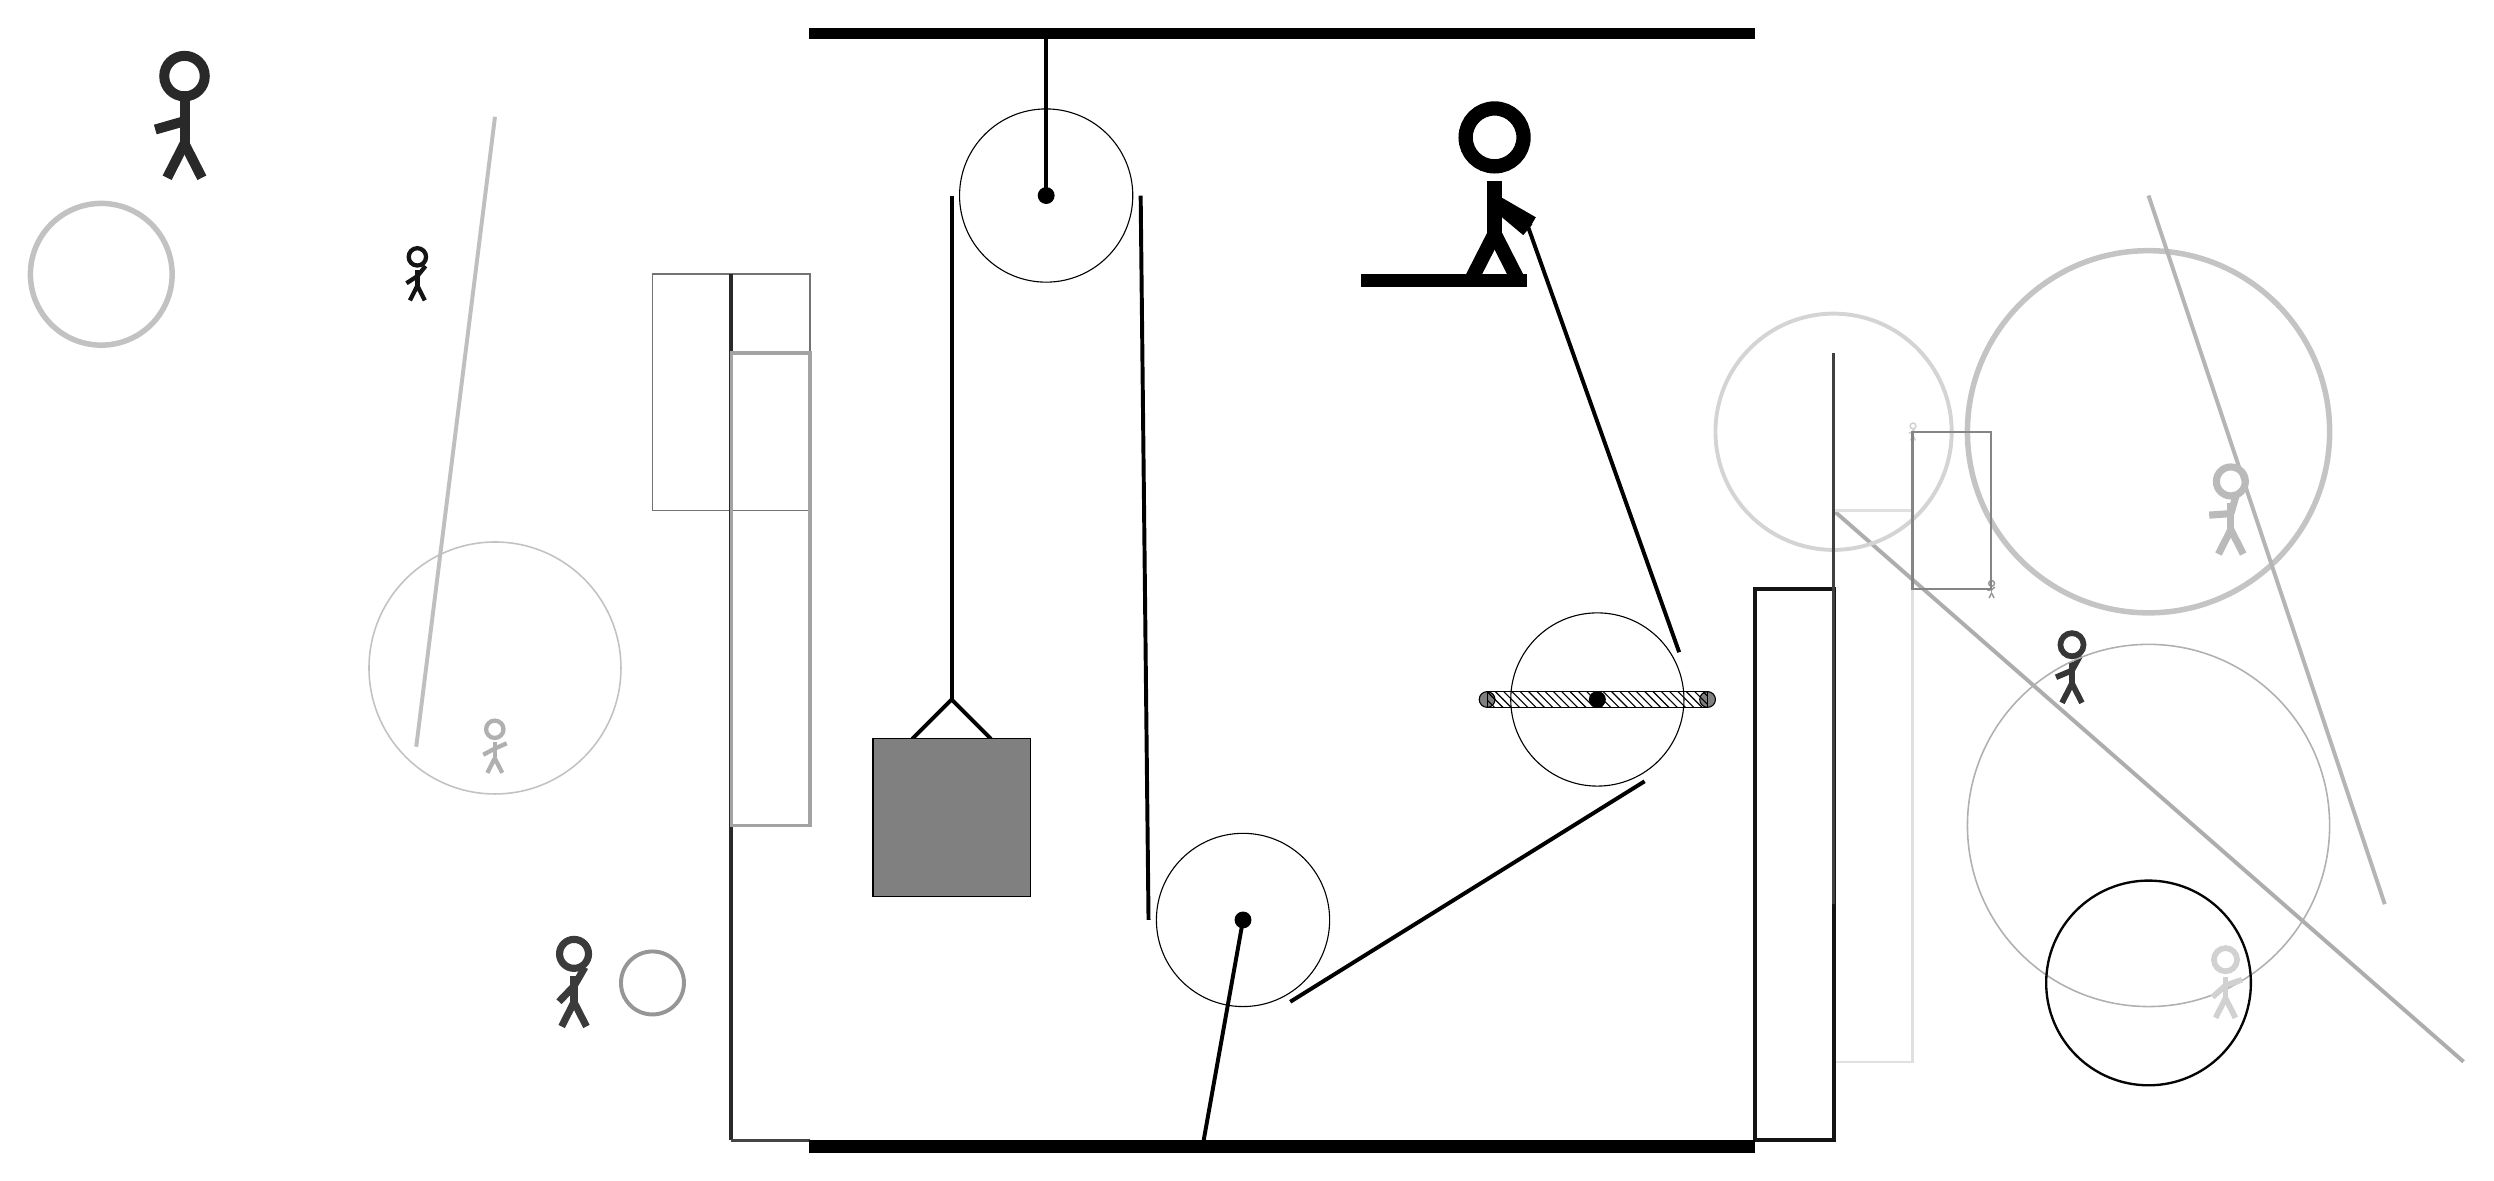
\begin{tikzpicture}
			%%%%% START %%%%%
			
			\draw[fill=black] (-2, 14) rectangle (10, 14.125);
			
			\draw[line width=0.5mm, color=black!32](11, 8) -- (19, 1);
			
			\draw [line width=0.7mm, color=black!23](15, 9) circle (2.3);
			\draw [line width=0.7mm, color=black!24](-11, 11) circle (0.9);
			\node[line width=0.3mm, color=black!19] at (12, 9) {\Strichmaxerl[1][8][73]};
			\node[line width=0.7mm, color=black!79] at (14, 6) {\Strichmaxerl[4][23][61]};
			
			\draw[line width=0.2mm, color=black!55] (-4, 11) rectangle (-2, 8);
			
			\draw[line width=0.5mm, color=black!29](15, 12) -- (18, 3);
			
			\node[line width=0.4mm, color=black!84] at (-10, 13) {\Strichmaxerl[7][16][90]};
			\draw [line width=0.2mm, color=black!31](15, 4) circle (2.3);
			
			\draw[line width=0.5mm, color=black!84](-3, 0) -- (-3, 11);
			
			\node[line width=0.2mm, color=black!41] at (13, 7) {\Strichmaxerl[1][5][42]};
			\draw [line width=0.5mm, color=black!17](11, 9) circle (1.5);
			\draw [line width=0.5mm, color=black!41](-4, 2) circle (0.4);
			\node[line width=0.4mm, color=black!18] at (16, 2) {\Strichmaxerl[4][42][19]};
			\node[line width=0.4mm, color=black!77] at (-5, 2) {\Strichmaxerl[5][46][60]};
			\draw[line width=0.3mm, color=black!73] (-3, 0) rectangle (-2, 0);
			
			\draw [line width=0.2mm, color=black!24](-6, 6) circle (1.6);
			\draw [line width=0.3mm, color=black!98](15, 2) circle (1.3);
			\node[line width=0.7mm, color=black!27] at (16, 8) {\Strichmaxerl[5][4][74]};
			
			\draw[line width=0.3mm, color=black!12] (12, 8) rectangle (11, 1);
			\node[line width=0.3mm, color=black!92] at (-7, 11) {\Strichmaxerl[3][33][51]};
			
			\draw[line width=0.5mm, color=black!92] (11, 0) rectangle (10, 7);
			\draw[line width=0.3mm, color=black!75] (11, 10) rectangle (11, 3);
			\draw[line width=0.3mm, color=black!48] (12, 9) rectangle (13, 7);
			\node[line width=0.2mm, color=black!31] at (-6, 5) {\Strichmaxerl[3][28][24]};
			
			\draw[line width=0.5mm, color=black!25](-7, 5) -- (-6, 13);
			\draw[line width=0.4mm, color=black!36] (-3, 4) rectangle (-2, 10);
			
			\draw (1, 12) circle (1.1);
			\draw[fill=black] (1, 12) circle (0.1);
			\draw[line width=0.5mm] (1, 14) -- (1, 12);
			
			\draw (3.5, 2.8) circle (1.1);
			\draw[fill=black] (3.5, 2.8) circle (0.1);
			\draw[line width=0.5mm] (3.5, 2.8) -- (3.0, 0);
			
			\draw[fill=white](8, 5.6) circle (1.1);
			\draw[fill=black] (8, 5.6) circle (0.1);
			\draw[fill=black!50] (9.4, 5.6) circle (0.1);
			\draw[fill=black!50] (6.6, 5.6) circle (0.1);
			\draw[pattern=north west lines, pattern color=black] (6.6, 5.7) rectangle (9.4, 5.5);
			
			\draw[line width=0.5mm](-0.7, 5.1) --  (-0.2, 5.6) -- (0.3, 5.1);
			\draw[fill=black!50] (-1.2, 5.1) rectangle (0.8, 3.1);
			
			\draw[line width=0.5mm](-0.2, 12) -- (-0.2, 5.6);
			\centerarc[line width=0.5mm](1, 12)(180:0:1.2000000000000002)
			\draw[line width=0.5mm](2.2, 12) -- (2.3, 2.8);
			\centerarc[line width=0.5mm](3.5, 2.8)(180:300:1.2000000000000002);
			\draw[line width=0.5mm](4.1, 1.7608) -- (8.6, 4.5608);
			\centerarc[line width=0.5mm](8, 5.6)(300:390:1.2000000000000002);
			\draw[line width=0.5mm](9.0392, 6.2) -- (7.05, 11.8);
			
			\node at (6.75, 12) {\Strichmaxerl[10][-220][-30]};
			\draw[fill=black] (5, 11) rectangle (7.1, 10.85);
			
			\draw[fill=black] (-2, 0) rectangle (10, -0.15);
			
			%%%%% END %%%%%
		\end{tikzpicture}
	\end{figure}	
\end{document}